\documentclass[10pt,twocolumn,letterpaper]{article}

\usepackage{cvpr}
\usepackage{times}
\usepackage{epsfig}
\usepackage{graphicx}
\usepackage{amsmath}
\usepackage{amssymb}
\usepackage[table,xcdraw]{xcolor}
\usepackage{adjustbox}
\usepackage{multirow}
\usepackage{floatrow}
\usepackage{booktabs}
\usepackage{float}
% Include other packages here, before hyperref.

% If you comment hyperref and then uncomment it, you should delete
% egpaper.aux before re-running latex.  (Or just hit 'q' on the first latex
% run, let it finish, and you should be clear).
\usepackage[breaklinks=true,bookmarks=false]{hyperref}
\DeclareMathOperator{\EX}{\mathbb{E}}% expected value

\cvprfinalcopy % *** Uncomment this line for the final submission

\def\cvprPaperID{12} % *** Enter the CVPR Paper ID here
\def\httilde{\mbox{\tt\raisebox{-.5ex}{\symbol{126}}}}

% Pages are numbered in submission mode, and unnumbered in camera-ready
\usepackage{xcolor} 
\usepackage{soul} 
\usepackage{xspace}
\usepackage{amsmath}
\DeclareRobustCommand{\mirco}[1]
{{\sethlcolor{cyan}\hl{#1}}} 

\usepackage{amssymb}% http://ctan.org/pkg/amssymb
\usepackage{pifont}% http://ctan.org/pkg/pifont

\newcommand{\cmark}{\ding{51}}%
\newcommand{\xmark}{\ding{55}}%

\usepackage{amsmath}
\DeclareMathOperator*{\argmax}{argmax} 

\definecolor{Green}{HTML}{AFDAAF}

\hyphenation{techniques}
\hyphenation{promote}
\hyphenation{cutting}

%\ifcvprfinal\pagestyle{empty}\fi
\setcounter{page}{1}
\begin{document}

%%%%%%%%% TITLE
\title{PoliTO-IIT Submission to the EPIC-KITCHENS-100 Unsupervised Domain Adaptation Challenge for Action Recognition}

\author{Chiara Plizzari{\thanks{The authors equally contributed to this work. This paper is partially supported by the ERC project RoboExNovo. We also acknowledge
that the research activity herein was carried out using the IIT
HPC infrastructure.}} $^{, 1}$ \quad
Mirco Planamente\footnotemark[1] $^{, 1,2}$ \quad 
Emanuele Alberti $^{1}$ \quad



Barbara Caputo\textsuperscript{1,2} \\


\and \textsuperscript{1} Politecnico di Torino\\
{\tt\small {name.surname}@polito.it}

\and \textsuperscript{2} Istituto Italiano di Tecnologia\\
{\tt\small {name.surname}@iit.it}
}

\maketitle
%\thispagestyle{empty}

\begin{abstract}
\label{sec:abstract}

%% 1. what is the problem 
Scientific applications that run on leadership computing facilities often face the challenge 
of being unable to fit leading science cases onto accelerator devices due to memory constraints 
(memory-bound applications).
%
% 2. what is your solution 
In this work, the authors studied one such US Department of Energy mission-critical condensed matter 
physics application, Dynamical Cluster Approximation (DCA++), and this paper discusses how device memory-bound challenges were successfully reduced  by proposing an effective 
``all-to-all'' communication method---a ring communication algorithm. 
%
This implementation takes advantage of acceleration on GPUs and remote direct memory access (RDMA) for fast data exchange between GPUs. 
%
\\Additionally, the ring algorithm was optimized with sub-ring communicators
and multi-threaded support to further reduce communication overhead and 
expose more concurrency, respectively.
%
% 3. What's the cherry-picked evaluation result you want to mention
The computation and communication were also analyzed 
by using the Autonomic Performance Environment for Exascale 
(APEX) profiling tool,  and this paper further discusses the 
performance trade-off for the ring algorithm implementation. 
%
The memory analysis on the ring algorithm shows that the allocation size for the authors' most 
memory-intensive data structure per GPU is now reduced to $1/p$ of the original size, where $p$ is the number of GPUs in the ring communicator.
%
The communication analysis suggests that 
the distributed Quantum Monte Carlo execution time grows linearly as sub-ring size increases, and the cost of messages passing through the network interface connector could be a limiting factor.


%
% \todoRed{Ronnie: Next sentence needs rewrite, too much information about Green's function that no one knows in the abstract; recommend generalizing.} \emph {However, DCA++ is currently facing memory-bound challenge as 
% a larger device array $G_t$ is limited by device memory size, where
% $G_t$ is a two-particle Green's function that allows condensed matter
% scientists to explore larger and more complex (higher fidelity)
% physics cases.}

\end{abstract}

\keywords{DCA++, Quantum Monte Carlo, GPU Remote Direct Memory Access, memory-bound issue, exascale machines}

\section{Introduction}
\label{sec:intro}

\subsection{Motivation}

Reliable estimation of a signal (or image) from nonlinear observations is of fundamental interest to several signal processing and machine learning applications. However, such an estimation is confounded by cases where the nonlinearity in each observation is well-modeled by a \emph{periodic} function such as a sinusoidal function, or sawtooth function, or a square-wave function. Periodic functions are many-to-one mappings, and inverting them can be challenging.

Our focus in this paper is a special kind of periodic nonlinear observation model encountered in high-dynamic range (HDR) imaging. It is well known that real world scenes contain a large range of brightness levels. However, due to hardware limitations, not all brightness levels can be accurately captured using conventional photography; if tuned incorrectly, most scene intensity levels can lie in the saturation region of the image sensors, causing loss of scene information. Similar problems arise in the case of multiplexed imaging systems, such as lensless and coded aperture imaging~\cite{codedaperture,asif2017flatcam}.

%While increasing the dynamic range can solve this problem, it is an impractical strategy since imaging sensors need to have infinite dynamic range, which is infeasible. 
One solution is to increase the dynamic range of the image sensors, but this can lead to expensive hardware. An alternative solution is to deploy a special type of image sensor that {wraps} the observed intensity value at a pixel over a given dynamic range. This is analogous to the familiar \emph{modulo} operation with respect to a parameter $R$, and we call this stylized imaging system a \emph{modulo camera}~\cite{ICCP15_Zhao}.  
Fig.~\ref{fig:func}(a) (black) depicts the modulo nonlinearity, and a major challenge is to undo the effect of this transformation for each observed pixel.

An added challenge in HDR imaging arises due to \emph{quantization}. In fact, the ``true" observations in a modulo camera are quantized versions of the (idealized) modulo observation, and the errors caused in the quantization propagates into the estimation process. Loss of information in the quantization process is unavoidable in principle, and the effect of quantization is magnified with fewer quantization levels. In acquisition systems with low bit-depth, such estimation errors can be very pronounced. Fig.~\ref{fig:func}(a) (cyan) depicts the quantization nonlinearity incurred during the observation process.

\subsection{Setup}

We formalize the above discussion as follows. Assume $\mathcal{X} \subseteq \R^{n}$ to be a given (known) subset in the data space, and consider a signal (or image) $x \in \mathcal{X}$. We model (possible) multiplexing operations and gain adjustments as linear transformations, denoted by $A\in\mathbb{R}^{p\times n}$ and $C\in\R^{m\times p}$ respectively. The composite observation model becomes:
\begin{equation}
\label{quan_obs}
u=f(Ax),~y=Q(Cu),
\end{equation}
where $f(\cdot)=\mod(\cdot,R)$ denotes the modulo function with respect to a range parameter $R$ and $Q(\cdot)$ denotes a quantization function. In this paper, we consider a 1-bit quantization function with only two levels, $0$ and $1$. A representative example is shown in Fig.\ \ref{fig:func} where $A$ and $C$ are identity operators. In  Figs~\ref{fig:func}(c)  and~\ref{fig:func}(d), the outputs of the functions $f$ and $Q$ are displayed when a test grayscale image (Fig.\ \ref{fig:func}(a)) is used in the input. Our overall objective is to estimate the original signal $x$ from the set of measurements $y$. 

%%%%%%%%%%%%%%%%%%%%%%%%%%%%%%%%%%%%%
\begin{figure}[t]
	
	\begin{center}
		\begingroup
		\setlength{\tabcolsep}{0.1pt} % Default value: 6pt
		\renewcommand{\arraystretch}{.1} % Default value: 1
		\begin{tabular}{ccc}      %{c@{\hskip .1pt}c@{\hskip .1pt}c}
			\multicolumn{3}{c}{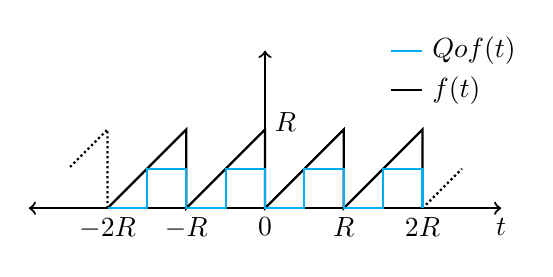
\begin{tikzpicture}
				\draw[<->,thick] (-3,0)--(3,0) node[anchor=north]{$t$};
				\draw (0,0) node[anchor=north]{$0$};
				\draw (0,1.1) node[anchor=west] {$R$};
				\draw (1,0) node[anchor=north]{$R$};
				\draw (2,0) node[anchor=north] {$2R$};
					\draw (-1,0) node[anchor=north]{$-R$};
				\draw (-2,0) node[anchor=north] {$-2R$};
				\draw[] (2,2) node[anchor=west] {{$Qof(t)$}};
				\draw[cyan,thick] (1.6,2) -- (2,2);
				%\draw [densely dotted,thick] (-2.5,1)--(3,1);
				\draw[->,thick] (0,0)--(0,2);
				\draw[] (2,1.5) node[anchor=west] {{$f(t)$}};
				\draw[thick] (1.6,1.5) -- (2,1.5);
				\draw[thick] (-2,0) --(-1,1)-| (-1,0) -- (0,1) -| (0,0) --(1,1)-| (1,0) -- (2,1) -| (2,0);
				\draw[densely dotted,thick] (2,0)--(2.5,0.5);
				\draw[densely dotted,thick] (-2,0)|-(-2,1) -- (-2.5,0.5);
				\draw[thick, cyan] (-2,0) -- ++(0.5,0)-| ++(0,0.5) -- ++(0.5,0) -| ++(0,-0.5) -- ++(0.5,0)-| ++(0,0.5) -- ++(0.5,0) -| ++(0,-0.5) -- ++(0.5,0)-| ++(0,0.5) -- ++(0.5,0) -| ++(0,-0.5) -- ++(0.5,0)-| ++(0,0.5) -- ++(0.5,0) -| ++(0,-0.5);
				\end{tikzpicture}}\\
			\multicolumn{3}{c}{(a)}\\
			\includegraphics[trim = 10mm 60mm 25mm 40mm,clip, width = 0.32\linewidth]{./orgimg.pdf}&
			\includegraphics[trim = 10mm 60mm 25mm 40mm,clip, width = 0.32\linewidth]{./modimg.pdf}&
			\includegraphics[trim = 10mm 60mm 25mm 40mm,clip,width = 0.32\linewidth]{./quantimg.pdf} \\
			(b) & (c) & (d)
		\end{tabular}
		\endgroup
	\end{center}
	\caption{\small{\emph{ (a) Modulo function, $f(t) = \mod(t,R)$ and quantized modulo function, $Qof(t)$; (b,c,d) Depiction of forward model. An input image (b) is transformed via a modulo function $f(t) = \mod(t,R)$, to (c). Such a ``modulo" image is further quantized to obtain (d).}}}
	\label{fig:func}
\end{figure}
%%%%%%%%%%%%%%%%%%%%%%%%%%%%%%%%%%%%%%%%%%%%%%%%%%

\subsection{Our contributions}

Clearly, the above estimation procedure is challenging due to the highly non-invertible nature of the observation model. In this paper, we design a systematic approach that takes some initial steps towards resolving this challenge. Our overarching assumption is that the measurement operations $A$ and $C$ are part of the design space. The core idea in our approach is that a very small, but carefully designed, non-adaptive set of measurements can support efficient estimation of the unknown signal.

Our approach follows stagewise. First, we consider the problem of inverting the quantization function, i.e., recovering $u$ from $y = Q(Cu)$. We demonstrate the existence of a linear operator $C$ (together with an efficient reconstruction algorithm) that supports such an inversion. Specifically, our operator $C$ obeys a particular block-diagonal form with weights chosen according to a harmonic progression; see Section~\ref{sec:Model} for details. We only consider 1-bit quantization functions, but similar ideas can presumably be extended for a higher number of quantization levels. In addition, our method supports the criterion of \emph{consistent reconstruction} as defined in \cite{jacques2011dequantizing}.

Next, we consider the problem of inverting the modulo operation, i.e., recovering $x$ from $u = f(Ax)$.  We propose an algorithm that builds upon the approach proposed in \cite{SoltaniHegde_ICASSP16}. In particular, we show that if the operator $A$ satisfies a certain \emph{factorization} $A = DB$, then $f$ can be stably inverted. To enable efficient inversion, the matrix $D$ must also be block-diagonal with weights chosen either randomly, or according to a geometric progression. In the former case, the reconstruction algorithm is an extension of the approach of~\cite{SoltaniHegde_ICASSP16}, while in the latter case the reconstruction follows the approach of~\cite{ICCP15_Zhao}.

The above two-stage procedure can be easily adapted to the case where we have some prior knowledge of the original signal $x$. This enables our approach to be used in conjunction with compressive imaging architectures. Common priors used in compressive imaging include \emph{sparsity} in some known orthonormal basis~\cite{foucart2013}. Note that our measurements are highly quantized and the total ``bit" complexity of our observations is far smaller than conventional techniques. Therefore, within our framework, one can choose to increase the number of quantizer measurements (rows of $C$) and/or modulo measurements (rows of $D$) in order to achieve better estimation performance.


Fig.~\ref{fig:demo} displays some representative results using our approach. We begin with a standard ``Peppers" image, compute a modulo transformation with three multiplexed measurements per pixel, and further modulate it with a sequence of three harmonic multipliers per measurement before passing it through a 1-bit quantizer. (In words, the overall ``oversampling factor" in our method is $9\times$.) The final binary measurements displayed in Fig.\ \ref{fig:demo}(a) are given as inputs to our reconstruction algorithm. The results from the first and second stages are displayed as images in Fig.\ \ref{fig:demo}(b). As is visually evident, our method is able to successfully reconstruct the image, as displayed in Fig.\ \ref{fig:demo}(c). 


\begin{figure}[t]
	\begin{center}
		\begingroup
		\setlength{\tabcolsep}{1pt} % Default value: 6pt
		\renewcommand{\arraystretch}{.1} % Default value: 1
		{\setlength{\tabcolsep}{1mm}
		\begin{tabular}{ccc|c|c}      %{c@{\hskip .1pt}c@{\hskip .1pt}c}
			\centering
			\includegraphics[trim = 30mm 60mm 40mm 65mm,clip, width = 0.15\linewidth]{./quant11.pdf}&
			\includegraphics[trim = 30mm 60mm 40mm 65mm,clip, width = 0.15\linewidth]{./quant12.pdf}&
			\includegraphics[trim = 30mm 60mm 40mm 65mm,clip, width = 0.15\linewidth]{./quant13.pdf}&
			\includegraphics[trim = 90mm 125mm 90mm 120mm,clip, width = 0.18\linewidth]{./mod11.pdf}&
				\multirow{3}{20mm}{\includegraphics[trim = 90mm 85mm 90mm 120mm,clip, width = \linewidth]{./dms_img.pdf}}\\
			\includegraphics[trim = 30mm 60mm 40mm 65mm,clip, width = 0.15\linewidth]{./quant21.pdf}& 
			\includegraphics[trim = 30mm 60mm 40mm 65mm,clip, width = 0.15\linewidth]{./quant22.pdf}&
			\includegraphics[trim = 30mm 60mm 40mm 65mm,clip, width = 0.15\linewidth]{./quant23.pdf}&
			\includegraphics[trim = 90mm 125mm 90mm 120mm,clip, width = 0.18\linewidth]{./mod21.pdf}&\\
			\includegraphics[trim = 30mm 50mm 40mm 65mm,clip, width = 0.15\linewidth]{./quant31.pdf}& 
			\includegraphics[trim = 30mm 50mm 40mm 65mm,clip, width = 0.15\linewidth]{./quant32.pdf}&
			\includegraphics[trim = 30mm 50mm 40mm 65mm,clip, width = 0.15\linewidth]{./quant33.pdf}& 
			\includegraphics[trim = 90mm 125mm 90mm 120mm,clip, width = 0.18\linewidth]{./mod31.pdf}&\\[1pt]
			\multicolumn{3}{c|}{(a)} &(b)&{\centering(c)}
		\end{tabular}}
		\endgroup
	\end{center}
	\caption{\small{\emph{Illustration of our approach. A given input image is modulated pixel-wise with three pre-chosen weights, passed through a modulo sensor, modulated again pixel-wise with three weights, and quantized to binary images. The resulting observations are shown in (a). The images in (b) and (c) represent the reconstruction of the modulo images, $\widehat{u}$ and the final image, $\widehat{x}$, respectively.}}}
	
	\label{fig:demo}
\end{figure}



\section{Our Approach}
In this section, we first describe the DG approach we used. %Indeed, the multi-source nature of the challenge setting make it perfect to deal with the domain shift using DG techniques, besides standard UDA ones. 
Then, we illustrate its extension to unlabelled target data under the standard UDA framework. Finally, we repurpose existing DA-based losses to induce consistency between different architectures. 

%and combine it with standard UDA techniques and we proposed new DA-based consistency losses. 
\subsection{Domain Generalization}
The multi-source nature of the proposed challenge setting makes it perfect to deal with the domain shift using DG techniques. %, besides standard UDA ones.
Thus, we first exploited a method which has been recently proposed to operate in this context, called Relative Norm Alignment (RNA) \cite{planamente2021crossdomain}.  %Indeed, the DG setting addresses the problem of learning a model able to generalize well by using inputs from multiple distributions, when no target data is available at all. 
This methods consists in performing an \textit{audio-visual domain alignment} at feature-level by minimizing a cross-modal loss function ($\mathcal{L}_{RNA}$). The latter aims at minimizing the \textit{mean-feature-norm distance} between the audio and visual features norms among all the source domains, %on multiple source domains to improve generalization ability of the network.%, 
and it is defined as
\begin{equation}\label{formula:rna_1}
    \mathcal{L}_{RNA}=\left(\frac{\EX[h(X^v)]}{\EX[h(X^a)]} - 1\right)^2,
\end{equation}
where $h(x^m_i)=({\lVert{ \cdot }\rVert}_2 \circ f^m)(x^m_i)$ indicates the $L_2$-norm of the features $f^m$ of the $m$-th modality, $\EX[h(X^m)]=\frac{1}{N}\sum_{x^m_i \in \mathcal{X}^m}h(x^m_i)$ for the $m$-th modality and $N$ denotes the number of samples of the set $\mathcal{X}^m=\{x^m_1,...,x^m_N\}$.

Authors of \cite{planamente2021crossdomain} proved that the norm unbalance between different modalities might cause the model to be biased towards the source domain that generate features with greater norm and thus causing a wrong prediction.  
Indeed, by simultaneously solving the problem of classification and relative norm alignment on different domains, the network extracts a shared knowledge between the different sources,  %learns features that are task-specific and meaningful to the final prediction, % to generate features with a similar norm, %and promotes those features that are task-specific and meaningful to the final prediction, 
resulting in a domain-agnostic model. 

In our submission to the EPIC-Kitchen UDA challenge, we extended the RNA-Net framework to the optical flow modality, and we exploited the multiple sources available from the official training splits to show the effectiveness of RNA loss in a multi-source DG setting. %The resulting loss combines an audio-visual alignment loss and a flow-visual ones, defined respectively as
%\begin{equation}\label{formula:rna_1}
%    \mathcal{L}^{av}_{RNA}=\left(\frac{\EX[h(X^v)]}{\EX[h(X^a)]} - 1\right)^2,
%\end{equation}
%\begin{equation}\label{formula:rna_2}
%    \mathcal{L}^{fv}_{RNA}=\left(\frac{\EX[h(X^v)]}{\EX[h(X^f)]} - 1\right)^2,
%\end{equation}
%where $h(x^m_i)=({\lVert{ \cdot }\rVert}_2 \circ f^m)(x^m_i)$ indicates the $L_2$-norm of the features $f^m$ of the $m$-th modality, $\EX[h(X^m)]=\frac{1}{N}\sum_{x^m_i \in \mathcal{X}^m}h(x^m_i)$ for the $m$-th modality and $N$ denotes the number of samples of the set $\mathcal{X}^m=\{x^m_1,...,x^m_N\}$. %The obtained results are shown in Table [REF]. [COMMENTO A TABELLA]

%\begin{itemize}
%    \item obiettivo produrre delle feat che sono meno dipendenti dal dominio 
%    sia perche riteniamo che questo allevia il secondo step (UDA) e sia perche permette di estrarre delle feature che sono migliori 
%    \item per questa parte abbiamo esteso il framework audio-visual proposto in (CITA-RNA) a lavorare anche con il flow. 
    
 %   \item tabellina piccola a tre righe solo su verb
 %   (source only baseline di EK, TA3N, our)
 
    
%\end{itemize}

\subsection{Domain Adaptation}
In this section, we describe the UDA techniques that are integrated in our approach.

\textbf{Relative Norm Alignment Network.} We followed the extension towards the UDA setting proposed in \cite{planamente2021crossdomain}, which is possible thanks to the unsupervised nature of RNA. %, taking also into account the Flow modality. 
In order to consider the contribution of both source and target data during training, we redefined $\mathcal{L}_{RNA}$ under the UDA setting as 

\begin{equation}\label{eq:loss_s_t}
    \mathcal{L}_{RNA}=\mathcal{L}^s_{RNA}+\mathcal{L}^t_{RNA} ,
\end{equation}
where $\mathcal{L}^s_{RNA}$ and $\mathcal{L}^t_{RNA}$ correspond to the RNA formulation in Equation \ref{formula:rna_1} illustrated above, when applied to source and target data respectively.

\textbf{Temporal Attentive Adversarial Adaptation Network (TA$^3$N).} Authors of \cite{videoda-chen2019temporal} proposed an UDA technique based on three components. The first one,  called \textit{Temporal Adversarial Adaptation Network (TA$^2$N)}, consists in an extension of DANN \cite{grl-pmlr-v37-ganin15}, %a standard adversarial UDA image-based method used to align the temporal features across domains.
aiming to align the temporal features on a multi-scale Temporal Relation Module (TRM) \cite{zhou2018temporal} through a gradient reversal layer (GRL).
%The domain alignment is obtained following the popular adversarial approach DANN [cita] on the multi-scale temporal relation module []. 
The second component is based on a domain attention mechanism which guides the temporal alignment towards features where the domain discrepancy is larger.
Finally, the third component uses a minimum entropy regularization (attentive entropy) to
refine the classifier adaptation.


%we add the minimum entropy regularization to
%refine the classifier adaptation. However, we only want to
%minimize the entropy for the videos that are similar across
%domains. Therefore, we attend to the videos which have
%low domain discrepancy, so that we can focus more on minimizing the entropy for these videos. 

\setlength\heavyrulewidth{0.31ex}

\begin{table*}[t]
\centering
\begin{adjustbox}{width=0.85\linewidth, margin=0ex 1ex 0ex 0ex}
\begin{tabular}{l|c|cccccc}
\toprule\noalign{\smallskip}
\multicolumn{8}{c}{\normalsize\textsc{Unsupervised Domain Adaptation Leaderboard}} \\
\noalign{\smallskip}
\cline{1-8}
\noalign{\smallskip}
  & Rank & \multicolumn{1}{c}{Verb Top-1} & Noun Top-1 & Action Top-1& Verb Top-5 & Noun Top-5 & Action Top-5\\ 
 \noalign{\smallskip} \hline
 chengyi        &1          & 53.16      & 34.86      & \textbf{25.00}        & 80.74      & 59.30      & 40.75        \\ \hline
M3EM             &2        & 53.29      & \textbf{35.64 }     & 24.76        & 81.64      & 59.89      & 40.73        \\ \hline
\rowcolor[HTML]{AFDAAF} 
 plnet        & 3            &\textbf{ 55.22}      & 34.83      & 24.71        & \textbf{81.93 }     & \textbf{60.48}      & \textbf{41.41}        \\ \hline
 EPIC\_TA3N \cite{damen2020rescaling}      & 6      & 46.91      & 27.69      & 18.95        & 72.70      & 50.72      & 30.53        \\ \hline
 EPIC\_TA3N\_SOURCE\_ONLY  \cite{damen2020rescaling} & 12 & 44.39      & 25.30      & 16.79        & 69.69      & 48.40      & 29.06   \\ 
\bottomrule
\end{tabular}
\end{adjustbox}
\caption{Leaderboard results of EPIC-Kitchens Unsupervised Domain Adaptation Challenge. The results obtained by the top-3 participants and the provided baseline methods are reported. \textbf{Bold:} highest result; {\color{Green}{\textbf{Green:}}} our final submission. }
\label{leaderboard}
\end{table*}

\setlength{\tabcolsep}{5pt}
\begin{table*}[t]
%\centering
%\RawFloats
\begin{minipage}{0.44\linewidth}
\begin{adjustbox}{width=1\linewidth, margin=0ex 0ex 0ex 0ex}
\begin{tabular}{l|ccc|ccc}
\toprule\noalign{\smallskip}
\multicolumn{7}{c}{\normalsize\textsc{Ensemble UDA losses}} \\
\noalign{\smallskip}
\cline{1-7}
\noalign{\smallskip}
   & \multicolumn{3}{c|}{Top-1} & \multicolumn{3}{c}{{Top-5}}\\ 
 \noalign{\smallskip}  \hline
 \noalign{\smallskip} 
  & \multicolumn{1}{c}{Verb} & Noun & Action & Verb  & Noun & Action \\  \hline \noalign{\smallskip}

{Ensemble}                       & 52.83      & 30.82      & 21.96        & \textbf{81.04}      & 52.67      & 46.66        \\ \hline \noalign{\smallskip}

Ensemble+T-HNA                 & 53.84      & 32.54      & 22.65        & 80.63      & 54.86      & 48.03        \\ \hline \noalign{\smallskip}

Ensemble+T-HNA+MEC & \textbf{54.02}      & \textbf{33.53 }     & \textbf{23.58 }       & 81.00      & \textbf{55.03}      & \textbf{48.27 }       \\ 
\bottomrule
\end{tabular}
\end{adjustbox}
%\end{table*}
\end{minipage}
\hspace{0.05\textwidth}
\centering
\begin{minipage}{0.35\linewidth}
\begin{adjustbox}{width=1\columnwidth, margin=0ex 0ex 0ex 0ex}
\begin{tabular}{l|ccc}
\toprule\noalign{\smallskip}
\multicolumn{4}{c}{\normalsize\textsc{Domain Generalization}} \\
\noalign{\smallskip}
\cline{1-4}
\noalign{\smallskip}
  & \multicolumn{1}{c}{Target} & Verb Top-1 & Verb Top-5 \\ 
 \noalign{\smallskip} \hline \noalign{\smallskip}

Source Only & \xmark               & 44.39 & 69.69 \\ \hline \noalign{\smallskip}

EPIC\_TA3N  \cite{damen2020rescaling}      & \cmark               & 46.91 & 72.70 \\ \hline \noalign{\smallskip}

RNA-Net \cite{planamente2021crossdomain}        & \xmark              & \underline{47.96} & \underline{79.54} \\ \hline
\noalign{\smallskip}
EPIC\_TA3N+RNA-Net    & \cmark               & \textbf{50.40} & \textbf{80.47} \\ 
\bottomrule
\end{tabular}
\end{adjustbox}
\caption{\textbf{Left.} Results on the EPIC-Kitchen validation set with different ensembling UDA losses. \textbf{Right.} Results on EPIC-Kitchen test set under the DG setting. \textbf{Bold} highest result. }
\label{multi-stream}
\end{minipage}
\end{table*}


\subsection{Ensemble UDA losses}

%Our idea is that by %directly combining different backbone
For our final submission, different models are used in order to exploit the potentiality of popular video architectures. 
Training individually each backbone with standard UDA protocols results in an adapted feature representation which varies from stream to stream. Our intuition is that this aspect could impact negatively the training process and the performance on target data. %cause an unbalance 
%during training, 
In fact, since the domain adaption process acts on each architecture independently, different prediction logits are obtained on target data. When combining them, this could cause a mismatch between the final scores, increasing the level of uncertainty of the model.
Thus, we impose a consistency constraint between feature representations from different models, by repurposing existing UDA loss functions to operate between multiple streams. Those are:

\textbf{Temporal Hard Norm Alignment (T-HNA).} It re-balances the contribution of each model during training by extending HNA \cite{planamente2021crossdomain} to align the norms of features coming from the different streams towards the same value $R$. This is applied on features extracted from multiple scales of each TRN module. The resulting $\mathcal{L}_\textit{T-HNA}$ is defined as
    
    \begin{equation}\label{eq:hna}
    \mathcal{L}_\textit{T-HNA}=\sum_b\left(\EX[h_t(X^b)] - R\right)^2,
\end{equation}
where $h_t$ denotes the $L_2$-norm of features extracted from the $t$-th multi-scale level of the $b$-th backbone network. 
    
\textbf{Min Entropy Consensus (MEC loss).} We extended the loss proposed in \cite{roy2019unsupervised} to encourage coherent predictions between different models. The resulting loss is defined as:
    \begin{equation}\label{eq:hna}
    \mathcal{L}_{MEC} = - \frac{1}{m}\sum_{i=1}^{m} \frac{1}{b} \max_{y \in \mathcal{Y} }{ \sum_{b} \mathrm{log} \textit{p}_b(y | x_{i}^{t})}
    \end{equation}
where $m$ is the cardinality of the batch size of the target set, $y$ is the predicted class, and $\mathrm{log} \textit{p}_b(y | x_{i}^{t})$ is the prediction probability of the $b$-th backbone network. The intuitive idea behind the proposed approach is to encourage different backbones to have a similar predictions.



\section{Framework}
In this section, we describe the architectures of the feature extractors used to produce suitable multi-modal video embeddings, and the fusion stategies adopted to combine them. We complete this section with the description of the hyper-parameters used for the training.

\subsection{Architecture}
\setlength\heavyrulewidth{0.31ex}

\textbf{Backbone.} %Our network is composed of three streams, one for each modality $m$, with distinct feature extractor $F^{m}$ and classifier $G^{m}$. 
For our submission, we adopted different network configurations.
In the first one, corresponding to the RNA-Net framework in \cite{planamente2021crossdomain}, %both the RGB and Flow streams 
we used the Inflated 3D ConvNet (I3D), pre-trained on Kinetics \cite{carreira2017quo}, for RGB and Flow streams, and a BN-Inception model \cite{ioffe2015batch} pre-trained on ImageNet \cite{imageNet} for the auditory information. % with a network initialized with ImageNet \cite{imageNet} pre-trained weights. 
Each feature extractor produces a 1024-dimensional representation which is fed to an action classifier. %$G^{m}$, consisting in a fully-connected layer that outputs the score logits. 
%Then, the two modalities are fused by summing the outputs and the cross entropy loss is used to train the network.
In the second configuration, we used BNInception for all the three streams, using pre-extracted features from a TBN \cite{munro2020multi} model trained on EPIC-Kitchens-55. In the last configurations, we used standard ResNet50 \cite{he2016deep} %and TSM[CITA] variation 
for all the streams using TSN \cite{wang2016temporal} and TSM~\cite{lin2019tsm} models pre-trained on Epic-Kitchen55\footnote{\url{https://github.com/epic-kitchens/epic-kitchens-55-action-models}}. 

\textbf{Multi-modal fusion strategies.}
In all the above mentioned configurations, each modality is processed by its own backbone, and the corresponding extracted representations are then fused following different strategies.
For RNA-Net, we followed a standard late fusion strategy, consisting in averaging the final score predictions obtained from two different fully-connected layers (verb, noun) from each modality. In the other configurations, we adopted the mid-fusion strategy proposed in \cite{Kazakos_2019_ICCV}, to generate a common frame-embedding among the modalities and used a Temporal Relation Module (TRM) \cite{zhou2018temporal} to aggregate features from different frames %obtaining with the 2D CNNs,
before feeding the final embeddings to the verb and noun classifiers.%In the other configurations, we adopt the mid-fusion strategy proposed in [cita], to generate a common frame-embedding among the modalities and used a Temporal Relation Module (TRM) \cite{zhou2018temporal} to aggregate features from different frames %obtaining with the 2D CNNs,
%before feeding the final embeddings to the two classifier. 

\setlength{\tabcolsep}{10pt}



\begin{table}[t]
\centering
\begin{adjustbox}{width=\columnwidth, margin=0ex 1ex 0ex 0ex}
\begin{tabular}{|c|c|c|c|c|c|}
\hline
$\lambda_{RNA}$ & $\lambda_{HNA}$ & $R$ & $\lambda_{MEC}$ & $\gamma$ & $\beta$         \\ \hline
1             & 0.0006        & 40         & 0.01                     & 0.003    & 0.75, 0.75, 0.5 \\ \hline
\end{tabular}
\end{adjustbox}
\caption{UDA losses hyper-parameters used during training.} %$\lambda_{RNA}$, $\lambda_{HNA}$ and $\lambda_{MCE}$ correspond to RNA, HNA and MCE losses weights respectively. $R$ corresponds to the radius value of HNA, and $\gamma$ and $\beta$ to TA$^3$N weights. }
\label{params}
\end{table}


\subsection{Implementation Details}
We trained I3D and BNInception models with SGD optimizer, with an initial learning rate of 0.001, dropout 0.7, and using a batch size of 128, following \cite{planamente2021crossdomain}. Instead, when using pre-extracted features from ResNet50 or BNInception, we trained the TRM modules on top of them for 100 epochs with an initial learning rate of 0.03, decayed after epochs 30 and 60 by a factor of 0.1. We used a batch size of 128 with SGD optimizer. In Table \ref{params} we report the other hyper-parameter used. Specifically, we indicate with $\lambda_{RNA}$, $\lambda_{T-HNA}$ and $\lambda_{MEC}$ the weights of RNA, T-HNA and MEC losses respectively, and with $R$ the values of the radius of T-HNA (see Equation \ref{eq:hna}). In addition, we report the values used in TA$^3$N to weight the attentive entropy loss ($\gamma$) and the domain losses at different levels ($\beta$). 
%The model of the first configuration are trained follow the same hyper-parameters used in [Cita]. Instead for the last three configuration, we train the models for 100 epochs with an initial learning rate of 0.01, decayed after 30 and 60 by a factor of 0.1. We used a batch size of 128 with SGD optimizer. 
%\mirco{vogliamo mettere una tabella riassuntiva dei pesi delle varie loss 1 RNA, 0.0006 HNR, 0.01ConsLoss, beta gamma ...}



\section{Results and Discussion}
%\begin{table}[t]
%\centering
%\begin{adjustbox}{width=0.75\columnwidth, margin=0ex 1ex 0ex 0ex}
%\begin{tabular}{l|ccc}
%\toprule\noalign{\smallskip}
%\multicolumn{4}{c}{\normalsize\textsc{Domain Generalization}} \\
%\noalign{\smallskip}
%\cline{1-4}
%\noalign{\smallskip}
%  & \multicolumn{1}{c}{Target} & Verb Top-1 & Noun Top-1 \\ 
% \noalign{\smallskip} \hline
%Source Only & \xmark               & 44.39 & 69.69 \\ \hline
%EPIC\_TA3N        & \cmark               & 46.91 & 72.70 \\ \hline
%RNA         & \xmark              & \underline{47.96} & \underline{79.54} \\ \hline
%EPIC\_TA3N+RNA    & \cmark               & \textbf{50.40} & \textbf{80.47} \\ 
%\bottomrule
%\end{tabular}
%\end{adjustbox}
%\caption{}
%\label{dg}
%\end{table}



% Please add the following required packages to your document preamble:
% \usepackage[table,xcdraw]{xcolor}
% If you use beamer only pass "xcolor=table" option, i.e. \documentclass[xcolor=table]{beamer}



In Table \ref{leaderboard} we report our best performing model on the target test, achieving the \textbf{1st} position on ‘verb', \textbf{3rd} on ‘noun' and ‘action', and \textbf{1st} position on Top-5 accuracy on all categories. In Table \ref{multi-stream} (left) we show an ablation on the contribution of the proposed ensemble UDA losses, T-HNA and MEC respectively, on the official validation set. As it can be seen, they improve Top-1 accuracy on all categories by up to $2\%$, proving the effectiveness of imposing a consistency between features from different streams. 

\textit{How well do DG approaches perform? } We show in Table \ref{multi-stream} (right) the results obtained under the multi-source DG setting, when target data are not available during training. Noticeably, RNA outperforms the baseline Source Only by up to $3\%$ on Top-1 and $10\%$ on Top-5, remarking the importance of using ad-hoc alignment techniques to deal with multiple sources in order to effectively extract a domain-agnostic model. Moreover, it outperforms the very recent UDA technique TA$^3$N without accessing to target data. 
Interestingly, when combined with EPIC\_TA3N, it further improves performance, proving the complementarity of RNA to other existing UDA approaches. 



{\small
\bibliographystyle{ieee_fullname}
\bibliography{egbib}
}

\end{document}
